\documentclass[border=3pt]{standalone}
% Preâmbulo compartilhado pelos diagramas TikZ da aula 8 de IHR (Métodos de Pesquisa)
\usepackage[T1]{fontenc}
\usepackage[utf8]{inputenc}
\usepackage{lmodern}
\usepackage{amsmath}
\usepackage{xcolor}
\usepackage{tikz}
\usetikzlibrary{arrows.meta,angles,quotes,decorations.pathmorphing,decorations.pathreplacing,calc,
                positioning,shapes.geometric,shapes.misc,backgrounds,fit,
                math}

% Paleta (mesma dos SVGs originais)
% Paleta da disciplina de IHR: acento azul (#1A6FB5), cor de destaque do tema.
% (o nome "dblue" é mantido para não alterar todos os diagramas)
\definecolor{dblue}{HTML}{1A6FB5}
\definecolor{dorange}{HTML}{B3541E}
\definecolor{dgreen}{HTML}{4A7C59}
\definecolor{dred}{HTML}{9C4B4B}
\definecolor{dcream}{HTML}{F4F1EA}
\definecolor{dshade}{HTML}{DDD7C9}

% Função gaussiana (não normalizada por padrão de escala visual)
\pgfmathdeclarefunction{gauss}{3}{%
  \pgfmathparse{1/(#3*sqrt(2*pi))*exp(-((#1-#2)^2)/(2*#3^2))}%
}

% Estilos comuns (prefixo d... para não colidir com chaves internas do pgf)
\tikzset{
  >={Stealth[length=2mm]},
  dguide/.style={gray!55, dashed, line width=0.4pt},
  daxis/.style={gray!60, line width=0.7pt, ->},
  dbody/.style={fill=black!3, draw=black!80, line width=1pt},
  dacc/.style={draw=dblue, line width=1pt},
  dlbl/.style={black!55, font=\small},
  dsub/.style={black!45, font=\footnotesize},
  dstate/.style={circle, draw=black!80, fill=dcream, line width=1pt,
                 minimum size=17mm, font=\large, inner sep=1pt},
  dobs/.style={circle, draw=black!80, fill=dshade, line width=1pt,
               minimum size=14mm, font=\large, inner sep=1pt},
  dbox/.style={rounded corners=2pt, draw=black!80, fill=dcream, line width=1pt,
               align=center, inner sep=6pt},
  dop/.style={circle, draw=black!80, fill=white, line width=1pt,
              minimum size=6mm, inner sep=0pt, font=\small},
  dtrans/.style={->, dblue, line width=1pt},
  dmeas/.style={->, dorange, line width=1pt},
  dcurve/.style={line width=1pt, dblue},
  dcurveb/.style={line width=1.4pt, dorange},
}

\begin{document}
\hyphenpenalty=10000 \exhyphenpenalty=10000 \tolerance=9999 \emergencystretch=3em
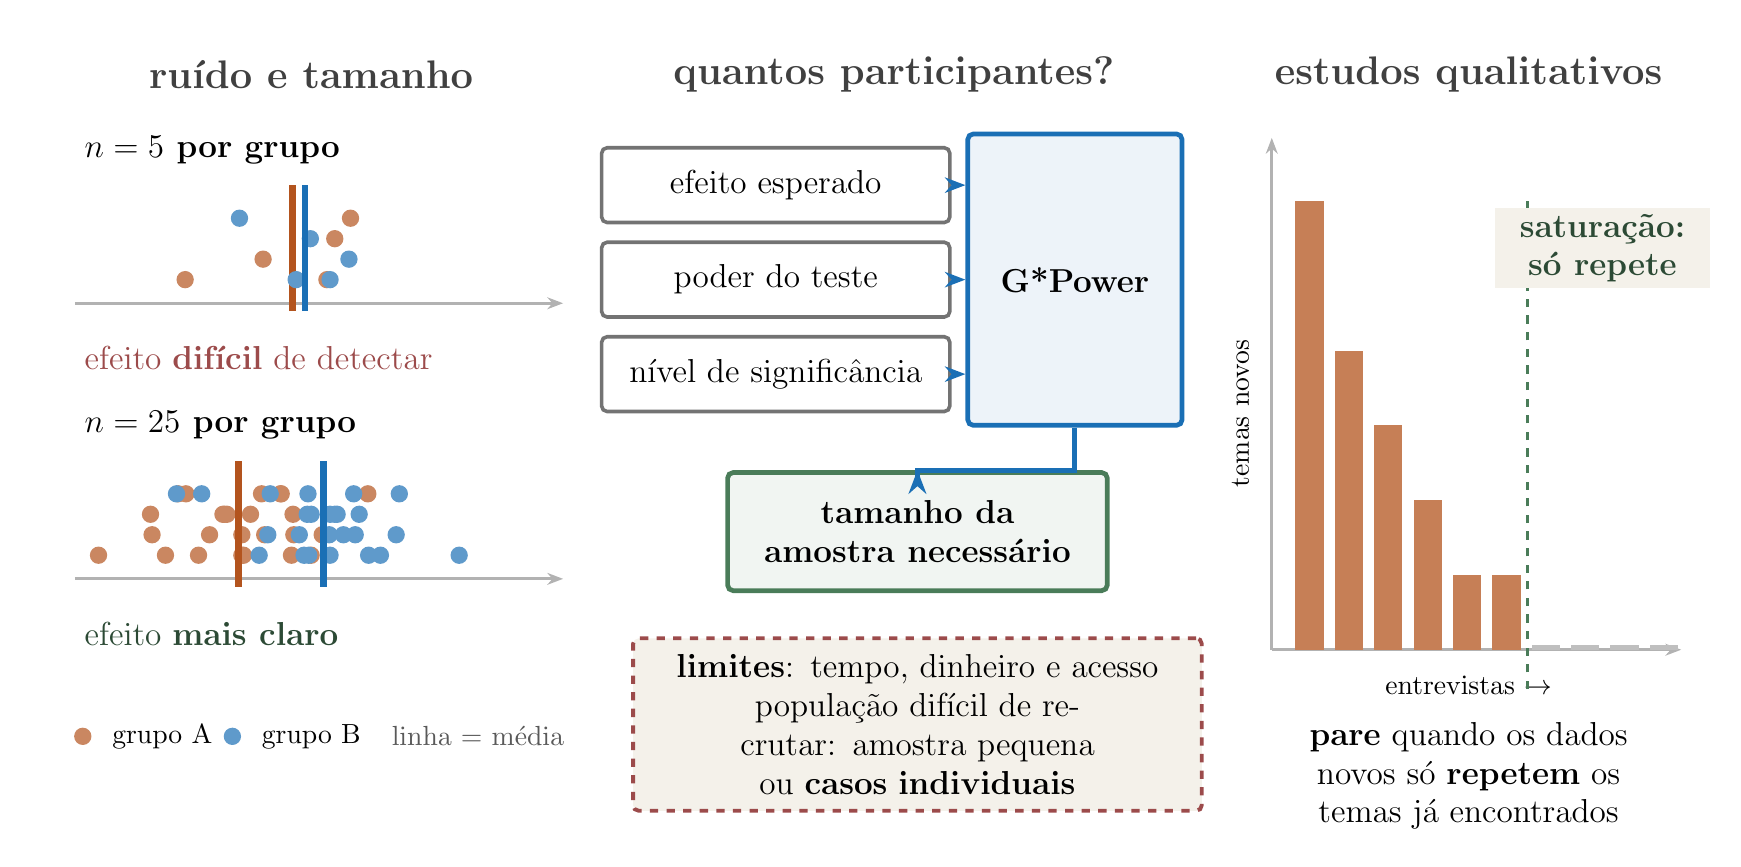
\begin{tikzpicture}[x=1cm,y=1cm]
  \useasboundingbox (-0.4,-0.9) rectangle (21.0,9.4);
  \node[font=\Large\bfseries, black!75] at (3.2,8.8) {ruído e tamanho};
  \draw[daxis, line width=1.1pt] (0.2,5.90) -- (6.4,5.90);
  \fill[dorange!70] (1.60,6.20) circle (0.11);
  \fill[dorange!70] (2.59,6.46) circle (0.11);
  \fill[dorange!70] (3.50,6.72) circle (0.11);
  \fill[dorange!70] (3.70,6.98) circle (0.11);
  \fill[dorange!70] (3.40,6.20) circle (0.11);
  \draw[dorange, line width=2.4pt] (2.96,5.80) -- (2.96,7.40);
  \fill[dblue!70] (3.44,6.20) circle (0.11);
  \fill[dblue!70] (3.68,6.46) circle (0.11);
  \fill[dblue!70] (3.19,6.72) circle (0.11);
  \fill[dblue!70] (2.29,6.98) circle (0.11);
  \fill[dblue!70] (3.01,6.20) circle (0.11);
  \draw[dblue, line width=2.4pt] (3.12,5.80) -- (3.12,7.40);
  \node[font=\large\bfseries, anchor=west] at (0.2,7.85) {$n=5$ por grupo};
  \draw[daxis, line width=1.1pt] (0.2,2.40) -- (6.4,2.40);
  \fill[dorange!70] (3.20,2.70) circle (0.11);
  \fill[dorange!70] (2.61,2.96) circle (0.11);
  \fill[dorange!70] (2.13,3.22) circle (0.11);
  \fill[dorange!70] (1.51,3.48) circle (0.11);
  \fill[dorange!70] (2.32,2.70) circle (0.11);
  \fill[dorange!70] (1.91,2.96) circle (0.11);
  \fill[dorange!70] (2.43,3.22) circle (0.11);
  \fill[dorange!70] (2.81,3.48) circle (0.11);
  \fill[dorange!70] (0.50,2.70) circle (0.11);
  \fill[dorange!70] (2.32,2.96) circle (0.11);
  \fill[dorange!70] (1.16,3.22) circle (0.11);
  \fill[dorange!70] (1.61,3.48) circle (0.11);
  \fill[dorange!70] (1.35,2.70) circle (0.11);
  \fill[dorange!70] (3.34,2.96) circle (0.11);
  \fill[dorange!70] (2.97,3.22) circle (0.11);
  \fill[dorange!70] (2.82,3.48) circle (0.11);
  \fill[dorange!70] (1.77,2.70) circle (0.11);
  \fill[dorange!70] (1.18,2.96) circle (0.11);
  \fill[dorange!70] (2.08,3.22) circle (0.11);
  \fill[dorange!70] (2.57,3.48) circle (0.11);
  \fill[dorange!70] (2.34,2.70) circle (0.11);
  \fill[dorange!70] (2.98,2.96) circle (0.11);
  \fill[dorange!70] (2.10,3.22) circle (0.11);
  \fill[dorange!70] (3.92,3.48) circle (0.11);
  \fill[dorange!70] (2.95,2.70) circle (0.11);
  \draw[dorange, line width=2.4pt] (2.28,2.30) -- (2.28,3.90);
  \fill[dblue!70] (5.08,2.70) circle (0.11);
  \fill[dblue!70] (3.61,2.96) circle (0.11);
  \fill[dblue!70] (3.20,3.22) circle (0.11);
  \fill[dblue!70] (2.68,3.48) circle (0.11);
  \fill[dblue!70] (4.08,2.70) circle (0.11);
  \fill[dblue!70] (4.28,2.96) circle (0.11);
  \fill[dblue!70] (3.53,3.22) circle (0.11);
  \fill[dblue!70] (3.74,3.48) circle (0.11);
  \fill[dblue!70] (3.17,2.70) circle (0.11);
  \fill[dblue!70] (3.05,2.96) circle (0.11);
  \fill[dblue!70] (3.15,3.22) circle (0.11);
  \fill[dblue!70] (1.81,3.48) circle (0.11);
  \fill[dblue!70] (2.54,2.70) circle (0.11);
  \fill[dblue!70] (3.43,2.96) circle (0.11);
  \fill[dblue!70] (3.50,3.22) circle (0.11);
  \fill[dblue!70] (4.32,3.48) circle (0.11);
  \fill[dblue!70] (3.93,2.70) circle (0.11);
  \fill[dblue!70] (3.76,2.96) circle (0.11);
  \fill[dblue!70] (3.44,3.22) circle (0.11);
  \fill[dblue!70] (1.49,3.48) circle (0.11);
  \fill[dblue!70] (3.44,2.70) circle (0.11);
  \fill[dblue!70] (2.65,2.96) circle (0.11);
  \fill[dblue!70] (3.81,3.22) circle (0.11);
  \fill[dblue!70] (3.16,3.48) circle (0.11);
  \fill[dblue!70] (3.11,2.70) circle (0.11);
  \draw[dblue, line width=2.4pt] (3.36,2.30) -- (3.36,3.90);
  \node[font=\large\bfseries, anchor=west] at (0.2,4.35) {$n=25$ por grupo};
  \node[font=\large, dred, anchor=west] at (0.2,5.2) {efeito \textbf{difícil} de detectar};
  \node[font=\large, dgreen!60!black, anchor=west] at (0.2,1.7) {efeito \textbf{mais claro}};
  \fill[dorange!70] (0.3,0.4) circle (0.11); \node[font=\normalsize, anchor=west] at (0.55,0.4) {grupo A}; \fill[dblue!70] (2.2,0.4) circle (0.11); \node[font=\normalsize, anchor=west] at (2.45,0.4) {grupo B}; \node[font=\normalsize, black!65, anchor=west] at (4.1,0.4) {linha = média};
  \node[font=\Large\bfseries, black!75] at (10.6,8.8) {quantos participantes?};
  \tikzset{ent/.style={dbox, draw=black!55, fill=white, line width=1.3pt, text width=4.0cm, minimum height=0.95cm, font=\large, align=center}}
  \node[ent] (a) at (9.1,7.4) {efeito esperado};
  \node[ent] (b) at (9.1,6.2) {poder do teste};
  \node[ent] (c) at (9.1,5.0) {nível de significância};
  \node[dbox, draw=dblue, fill=dblue!8, line width=1.7pt, text width=2.3cm, minimum height=3.7cm, font=\large\bfseries, align=center] (g) at (12.9,6.2) {G*Power};
  \draw[dtrans, line width=1.6pt, -{Stealth[length=2.6mm]}] (a.east) -- (g.west |- a.east);
  \draw[dtrans, line width=1.6pt, -{Stealth[length=2.6mm]}] (b.east) -- (g.west |- b.east);
  \draw[dtrans, line width=1.6pt, -{Stealth[length=2.6mm]}] (c.east) -- (g.west |- c.east);
  \node[dbox, draw=dgreen, fill=dgreen!8, line width=1.7pt, text width=4.4cm, minimum height=1.5cm, font=\large\bfseries, align=center] (t) at (10.9,3.0) {tamanho da amostra necessário};
  \draw[dtrans, line width=1.8pt, -{Stealth[length=3mm]}] (g.south) -- ++(0,-0.55) -| (t.north);
  \node[dbox, draw=dred, dashed, line width=1.4pt, text width=6.8cm, minimum height=1.9cm, font=\large, align=center] at (10.9,0.55) {\textbf{limites}: tempo, dinheiro e acesso\\ população difícil de recrutar: amostra pequena ou \textbf{casos individuais}};
  \node[font=\Large\bfseries, black!75] at (17.9,8.8) {estudos qualitativos};
  \draw[daxis, line width=1.2pt] (15.4,1.5) -- (20.6,1.5); \draw[daxis, line width=1.2pt] (15.4,1.5) -- (15.4,8.0);
  \fill[dorange!75] (15.70,1.5) rectangle (16.06,7.20);
  \fill[dorange!75] (16.20,1.5) rectangle (16.56,5.30);
  \fill[dorange!75] (16.70,1.5) rectangle (17.06,4.35);
  \fill[dorange!75] (17.20,1.5) rectangle (17.56,3.40);
  \fill[dorange!75] (17.70,1.5) rectangle (18.06,2.45);
  \fill[dorange!75] (18.20,1.5) rectangle (18.56,2.45);
  \fill[black!25] (18.70,1.5) rectangle (19.06,1.56);
  \fill[black!25] (19.20,1.5) rectangle (19.56,1.56);
  \fill[black!25] (19.70,1.5) rectangle (20.06,1.56);
  \fill[black!25] (20.20,1.5) rectangle (20.56,1.56);
  \node[font=\normalsize, rotate=90] at (15.0,4.5) {temas novos};
  \node[font=\normalsize] at (17.9,1.05) {entrevistas $\rightarrow$};
  \draw[dgreen, dashed, line width=1.3pt] (18.65,1.0) -- (18.65,7.2);
  \node[font=\large\bfseries, dgreen!60!black, text width=2.6cm, align=center, fill=dcream, inner sep=2pt] at (19.6,6.6) {saturação:\\ só repete};
  \node[font=\large, text width=5.4cm, align=center] at (17.9,-0.1) {\textbf{pare} quando os dados novos só \textbf{repetem} os temas já encontrados};
\end{tikzpicture}
\end{document}
